\documentclass[a4paper, 12pt]{article}
\usepackage[hmargin=2cm,vmargin=2.5cm]{geometry}
\usepackage{enumerate}
\usepackage{makecell}
\usepackage{graphicx}
\usepackage{hyperref}
\usepackage{amsmath}
\usepackage[table]{xcolor}
\usepackage{minted}
\usepackage{graphicx}
\usepackage[french]{babel}
\usepackage[utf8]{inputenc}
\usepackage[T1]{fontenc}
\usepackage[
    backend=biber,
    style=alphabetic,
    sorting=none
]{biblatex}

\usepackage{biblatex}
\usepackage{url}
\addbibresource{Reference.bib}

\usepackage{enumitem}
\usepackage{xcolor}
\usepackage{fancyhdr}
\usepackage{titlesec}
\usepackage{comment}
\usepackage{listings}

%------------to insert python code-----------------
\lstnewenvironment{Pythoncode}[1][]
  {\lstset{
    language=Python,
    basicstyle=\small\ttfamily,
    keywordstyle=\color{blue},
    stringstyle=\color{red},
    commentstyle=\color{green!60!black},
    numbers=left,
    numberstyle=\tiny\color{gray},
    breaklines=true,
    showstringspaces=false,
    captionpos=b,
    frame=single,
    #1
  }}
  {}

  
\hypersetup{
    colorlinks,
    citecolor=black,
    filecolor=black,
    linkcolor=black,
    urlcolor=black
}
\begin{comment}
    \setlength{\arrayrulewidth}{0.4mm}
    \newcommand{\HRule}{\rule{\linewidth}{0.5mm}}
    
    \pagestyle{fancy}
    \fancyhead[R]{\textbf{\textcolor{cyan}{SI-CRYPTOGRAPHIE}}\\
    \textbf{\textcolor{cyan}{MAC}}}
\end{comment}

\setlength{\arrayrulewidth}{0.4mm}
\newcommand{\HRule}{\rule{\linewidth}{0.5mm}}

\pagestyle{fancy}
\fancyhead[R]{\textbf{\textcolor{cyan}{SI-CRYPTOGRAPHIE}}\\
\textbf{\textcolor{cyan}{MAC}}}

%-----to set the spacing for all sections and subsections in the document-------------
\titlespacing{\section}{0pt}{\baselineskip}{\baselineskip}
\titlespacing{\subsection}{0pt}{\baselineskip}{\baselineskip}


\begin{document}
\begin{titlepage}
  \begin{center}
    % logo
    
\includegraphics[width=0.20\textwidth]{Sections/Images/LOGO.jpg}~\\[1cm]

    \textsc{\Large DEPARTEMENT DU GENIE INFORMATIQUE\\ ECOLE NATIONALE SUPERIEURE POLYTECHNIQUE DE YAOUNDE}\\[3cm]


    \HRule \\[0.4cm]
    {\large \bfseries SYSTEME D'INFORMATION(CRYPTOGRAPHIE): \\ MESSAGE AUTHENTIFICATION CODE (MAC)\\[0.4cm]}
    \HRule \\[4cm]
    \large\textbf{\underline{Etudiants:}}\\NGHOGUE TAPTUE FRANCK RODDIER(21P279)\\NGO BASSOM ANNE ROSALIE(21P089)\\ NTYE EBO'O NINA LAISSA(21P223)\\MBIAMY NGAMENI STEVEN LOIC(23P770)\\ KOGHENE LADZOU ERIC(23P752)\\[3cm]

    \vfill
   {\large \underline{Sous la supervision de}: \textbf{Dr. TALE KALACHI HERVE}}

  \end{center}
\end{titlepage}


%-------------Creating the table of content------------------------
\tableofcontents

\begin{center}\textbf{INTRODUCTION}
\end{center}

Depuis l'apparition d'internet, il est possible de communiquer d'un bout à l'autre de la planète. Cependant, en même temps que ce dernier, sont apparus de nombreux vices, plus connus sous le nom de cybercriminalité. Face à cette menace, il s’est très vite imposé le besoin de garantir l’authenticité et l'intégrité des informations échangées sur Internet. \\
En fait, ce besoin remonte à plus loin, dès l'époque où l'Homme a été capable de communiquer. Par exemple, pendant la seconde guerre mondiale, les puissances impliquées ont dû mettre en jeu de nombreux stratagènes cryptographiques dans le but de garantir l'intégrité et l'authenticité des informations qu'elles recevaient. Dès lors, les MACs(Message Authentification Codes) se sont imposés comme une solution inncontournable pour satisfaire ce besoin. \\
Le but de cet exposé sera donc de nous permettre, futurs ingénieurs informaticiens, de comprendre le fonctionnnement des MACs et ainsi de garantir l'intégrité et l'authenticité des informations qui seront amenées à circuler dans les systèmes d'information que nous serons amenés à mettre ne place dans l'avenir.

\newpage

\section{\textbf{\underline{INTRODUCTION AU MAC}}}
\subsection{\textbf{\underline{DEFINITION DU MAC}}}

Un \textbf{code d'authentification de message}, de l'anglais Message Authentification Code, en abrégé \textbf{MAC}, est une valeur calculée à partir d'un message et d'une \textbf{clé secrète partagée entre l'émetteur et le destinataire du message}. Ce MAC est ensuite envoyé avec le message au destinataire, et le destinataire peut le vérifier en utilisant la même clé et la même fonction de calcul que l'émetteur.

Le MAC est un outil essentiel dans le domaine des correspondances secrètes en ce sens qu'il permet de garantir deux des qualités d'une bonne information (dans ce cas l'information portée par le message):
\begin{itemize}[label=$\cdot$]
    \item \textbf{L'intégrité} : En fait l'algorithme de calcul d'un MAC donne des résultats différents si on change le contenu du message, ce qui permet d'éviter en général la modification du message, et dans d'autres cas d'aviser le destinataire d'une quelconque modification de son message.
    \item \textbf{L'authenticité} : De même, il  donne des résultats différents si on change l'émetteur et/ou le destinataire du messages, ce qui permet ainsi d'éviter les usurpations d'identité.
\end{itemize}
\subsection{\textbf{\underline{FONCTIONNEMENT DU MAC}}}

Le principe de fonctionnement des MACs est plutôt simple, en ce sens qu'il s'agit pour l'émetteur :
\begin{itemize}[label=$\cdot$]
    \item D'écrire le message.
    \item De calculer son MAC à l'aide de l'algorithme de calcul et de la clé secrète qu'il a en commun avec le destinataire.
	\item D'envoyer le MAC et le message au destinataire.
\end{itemize}
Pour le destinataire:
\begin{itemize}[label=$\cdot$]
    \item Une fois le message reçu, le destinataire calcule son MAC à l'aide de la clé secrète qu'il a en commun avec l'émetteur.
    \item Il compare le résultat obtenu avec le MAC envoyé par l'émetteur: En cas d'égalité, le message est authentique et intègre, par contre, s'il est  diffèrent, il est soit corrompu soit non authentique.
\end{itemize}

\begin{center}
\textbf{Schema illustratif de la situation}:\newline \newline

    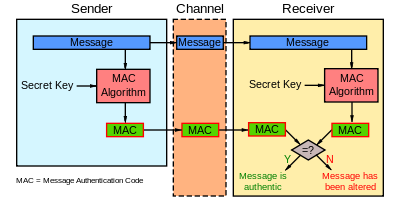
\includegraphics[width=10cm, height=5cm]{Sections/Images/fonctionnement.png}
\end{center}

Nous venons de presenter de facon generale ce qu'est le MAC, afin de faciliter la comprehension de la chose nous allons passer a une illustration.

Supposons que un général de l'armée Française veuille envoyer une demande de renforts au général de l'armée Anglaise mais ne veut pas que son message soit corrompu:

-	Il commence par écrire son message M : "Ici France, demande renforts en urgence"
-	Il calcule son MAC avec l'algorithme de calcul G et la clé secrète K\\
G(M, K) = 0101010101010001111100101001001110010 (par exemple)\\
-	Il envoie ensuite son message et son MAC au général Anglais (il peut décider de crypter son message ou  non, cela ne nous intéresse pas)
-	Le général Anglais reçoit le message et le MAC (il décrypte le message si nécessaire
-	Il recalcule le MAC à partir du message qu'il a reçu, de l'algorithme de calcul et de sa clé secrète commune avec le général Français et il le compare au MAC reçu, par exemple il reçoit M:"Ici France, demande renforts en urgence" et il calcule le MAC :\\
G(M, K) = 0101010101010001111100101001001110010\\ les MACs sont identiques, donc il peut se fier au message
Imaginons que le message ait été modifié par le général Allemand et que le général Anglais reçoit plutôt M' : "Ici France, vous les Anglais être poules mouillées, laissez nous gérer cette guerre tous seuls, bande de faibles", il calcule le MAC et obtient:\\
G(M', K) = 1100101101001011010111011001101000111 (par exemple)\\ les MACs sont différents, il sait qu'il ne peut pas se fier au message et il recherche un moyen de s'entendre avec la France sur un autre moyen de communication.

\subsection{\textbf{\underline{CHOIX DE LA CLE SECRETE}}}
Dans le contexte du code d'authentification de message (MAC), la clé secrète utilisée pour la génération et la vérification des MACs est généralement générée à l'aide d'un processus de génération de clé sécurisé. L'échange sécurisé de la clé secrète peut être réalisé à travers diverses méthodes, telles que des protocoles d'établissement de clé ou des mécanismes de distribution de clé sécurisés.

Voici un aperçu général de la génération de clé secrète et de l'échange sécurisé dans les systèmes MAC :

\begin{enumerate}
    \item \textbf{Génération de clé secrète }: La clé secrète joue un rôle essentiel dans les algorithmes MAC. Il s'agit d'un secret partagé connu uniquement des entités impliquées dans la communication.\\\\
    La clé secrète doit être générée à l'aide d'un \textbf{générateur de nombres aléatoires cryptographiquement sécurisé} (CSPRNG) pour garantir une entropie suffisante et une résistance aux attaques par force brute.\\\\
    Selon l'algorithme MAC spécifique et ses exigences, la longueur de la clé peut varier. Il est essentiel d'utiliser une longueur de clé offrant un niveau de sécurité adéquat.
    
    \item \textbf{Échange sécurisé de clé} : L'échange sécurisé de la clé secrète entre les parties communicantes est crucial pour maintenir la confidentialité et l'intégrité du MAC.\\\\
    Des protocoles d'établissement de clé, tels que l'échange de \textbf{clés Diffie-Hellman} accompagné par la \textbf{signature numérique} (pour vérifié la non répudiation), peuvent être utilisés pour établir une clé secrète partagée de manière sécurisée sur un canal non sécurisé.\\\\
    Alternativement, si les parties communicantes partagent déjà un canal sécurisé (par exemple, une connexion sécurisée préétablie ou un environnement physiquement sécurisé), elles peuvent échanger la clé secrète directement via ce canal.\\
    
    \item \textbf{Distribution de clé} : Dans certains cas, une tierce partie de confiance peut être impliquée dans la distribution sécurisée de la clé secrète aux parties communicantes.\\\\
    Des mécanismes de distribution de clé, tels que des \textbf{protocoles de gestion de clé} ou des \textbf{centres de distribution de clé}, peuvent être utilisés pour distribuer la clé secrète de manière sécurisée aux destinataires prévus.\\\\
    La tierce partie de confiance veille à ce que la clé secrète soit transmise de manière sécurisée à chaque partie sans interception ni altération.
    \newline \newline \newline
\end{enumerate}


\subsection{\textbf{\underline{Référence de cette partie}}}
\begin{center}
    \cite{wiki:mac}\\
    \cite{openclassrooms:mac}\\
    \cite{principe:mac}\\
    \cite{saied2014lightweight}\\
    \cite{dasari2015random}\\
    \cite{boumso2006methode}\\
\end{center}

\section{\textbf{\underline{METHODES DE CONSTRUCTION DES MACs}}}
\subsection{\textbf{\underline{CONSTRUCTION A BASE DES BLOCS CHIFFRES}}}

Les blocs chiffrés sont des algorithmes de chiffrement symétrique qui opèrent sur des blocs de données de taille fixe, généralement de 64 ou 128 bits. Ils utilisent une clé secrète pour transformer le bloc de données en un bloc chiffré. Les blocs chiffrés sont utilisés pour assurer la confidentialité des messages, mais ils peuvent aussi servir à construire des MACs. Pour cela, il faut combiner les blocs chiffrés avec un mode opératoire, qui définit comment les blocs du message sont traités et reliés entre eux. Il existe plusieurs modes opératoires possibles, qui ont des propriétés et des performances différentes. Les plus connus sont le CBC-MAC et le C-MAC.

\subsubsection{\textbf{\underline{LE CBC-MAC}}}

CBC MAC est une fonction à base de blocs chiffrés qui utilise le \textbf{mode CBC (Cipher Block Chaining)} pour chiffrer le message avec la clé secrète. Le MAC est le dernier bloc chiffré obtenu par ce mode. Il a été inventé en \textbf{1981} par \textbf{John Black, Phillip Rogaway et Thomas Shrimpton}. Son principe de fonctionnement est le suivant :

\begin{itemize}
    \item [\textbullet] Le message est divisé en blocs de meme taille, par exemple \textbf{128 bits ou 64 bits}, selon la méthode de chiffrement par blocs utilisé. On ajoute du \textbf{paddding} au message pour compléter le dernier bloc.
    \item [\textbullet] On choisit aléatoirement un \textbf{vecteur d'initialisation (IV)}, il doit etre de meme taille que les blocs du message. L'IV n'est pas secret, il peut etre envoyé avec le message et le MAC.
    \item [\textbullet] On chiffre le premier bloc du message avec la clé secrète en utilisant un algorithme de chiffrement par bloc (généralement AES ou DES). On obtient un premier bloc chiffré.
    \item [\textbullet] On effectue une opération XOR entre le premier bloc chiffré et le deuxième bloc du message. Puis on utilise le resultat de cette operation pour chiffrer le deuxieme bloc du message grace a l'algorithme de chiffrement par bloc et de la meme cle k.
    \item [\textbullet] On repète l'opération XOR et le chiffrement pour tous les blocs du message, en utilisant à chaque fois le meme algorithme de chiffrement par blocs. On obtient ainsi une chaine de blocs chiffrés.
    \item [\textbullet] Le MAC est le dernier bloc chiffré de la chaine.
\end{itemize}

\begin{center}
    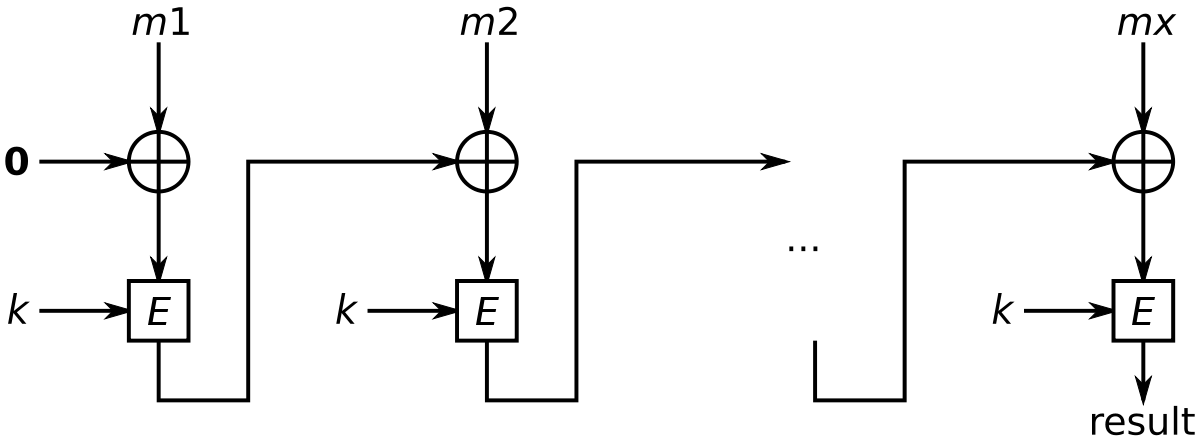
\includegraphics[width=10cm, height=7cm]{Sections/Images/CBC.svg.png}
\end{center}


LE CBC MAC présente tout de meme des failles, les plus connus sont celles de \textbf{l'attaque de Preneel et Van Oorschot, et l'insécurité avec des message de taille vairiable}.\\ 

\textbf{Attaque de Preneel et Van Oordchot}\\

L'attaque décrite par Preneel et Van Oorschot permet de forger des codes d'authentification pour des messages arbitraires sans avoir besoin de connaitre la clé secrète. Pour etre réalisé, l'attaquant a besoin d'environ  $2^{n/2}$ textes connus accompagnés de leurs MACs, forgé avec la clé secrète, où n est la longueur du bloc en bits. L’attaque se déroule comme suit:


\begin{itemize}
    \item [\textbullet] L’attaquant collecte $2^{n/2}$ paires $(M_i, T_i)$, ou $M_i$ est un message de longueur fixe et $T_i$ est son code d’authentification calculé avec le CBC-MAC et la clé secrète k.
    \item [\textbullet] L’attaquant trie les paires selon la valeur de $T_i$ et cherche deux paires $(M_i, T_i)$ et $(M_j, T_j)$ telles que $T_i = T_j$. Il y a une probabilité d’environ $50\%$ qu’il en trouve, selon le paradoxe des anniversaires.
    \item [\textbullet] L’attaquant construit un nouveau message $M = M_i || M_j'$, où $M_j'$ est le message $M_j'$ auquel on a retiré le premier bloc. Le code d’authentification de M est alors $T_j$, car le CBC-MAC de $M_j’$ est égal au CBC-MAC de $M_i$. L’attaquant a donc réussi à forger un code d’authentification sans connaître la clé secrète k.\\
\end{itemize} 

\textbf{Solutions pour renforcer le CBC-MAC}\\

Pour pallier aux limites du CBC-MAC, plusieurs solutions ont été imaginés telles que:

\begin{itemize} 
    \item [\textbullet] Utiliser des clés différentes pour le chiffrement et le code MAC, afin d’éviter les interférences entre les deux opérations
    \item [\textbullet] Utiliser des clés dérivées de la clé principale pour chaque longueur de message possible, afin d’éviter les attaques par concaténation.
    \item [\textbullet] Ajouter un bloc final contenant la longueur du message, afin de distinguer les messages de taille variable.
    \item [\textbullet] Utiliser des variantes du CBC-MAC, comme le CMAC, qui utilise des opérations supplémentaires pour éviter les collisions entre les codes d’authentification.
\end{itemize}
\subsubsection{\textbf{\underline{Le C-MAC}}}

Le \textbf{C-MAC} est une variante du CBC-MAC qui utilise 2 clés secrètes : Une fois le MAC obtenu avec CBC, il suffit de le rechiffrer avec la deuxième clé secrète. Les deux cles sont obtenus en utilisant la cle secrete et une derivation key qui est au prealable passe dans une fonction appelee key derivation function qui permet de dupliquer et d'obtenir deux cles pseudo-aleatoirement.Avec la premiere cle on effectuera le meme procede que celui du CBC MAC et pour chiffrer le deuxieme bloc on utilise la deuxieme cle.

\newpage
\subsection{\textbf{\underline{CONSTRUCTION A BASE DE FONCTIONS DE HACHAGE}}}

Les \textbf{fonctions de hachage} sont des fonctions mathématiques qui transforment un message de taille arbitraire en une valeur fixe, appelée \textbf{empreinte ou digest}.Elles sont aussi utilisés pour calculer les MACs, pour cela on il faut les combiner avec une clé secrète. La méthode de construction des MACs utilisant une fonction de hachage la plus connue est le H-MAC, mais il existe aussi d'autres méthodes comme le N-MAC.

 \subsubsection{\textbf{\underline{Le H-MAC}}}

\textbf{HMAC} (Keyed-Hash Message Authentication Code) est un algorithme cryptographique largement utilisé qui assure l'authentification et l'intégrité des messages et a été proposé en 1997 par \textbf{Bellare}, \textbf{Canetti}, and \textbf{Krawczyk} dans l'article \textbf{"Keying Hash Functions for Message Authentication."}\\\\
Il repose sur le concept d'utilisation \textbf{d'une fonction de hachage cryptographique en combinaison avec une clé secrète pour générer un code d'authentification de message (MAC)}.\\

L'algorithme HMAC peut être défini comme suit :\\
\begin{enumerate}
    \item \textbf{Sélection d’une fonction de Hachage}\\Sélectionnez une fonction de hachage cryptographique appropriée, telle que MD5, SHA-1 ou SHA-256. Le choix de la fonction de hachage dépend du niveau de sécurité souhaité et des exigences spécifiques de l'application.\\
    \item \textbf{Choix d’une clé secrète}\\Choisissez une clé secrète connue uniquement de l'expéditeur et du destinataire. La longueur de la clé doit être adaptée à la fonction de hachage choisie. Une clé plus longue offre une meilleure sécurité mais peut également affecter les performances.\\
    \item \textbf{Calcule du HMAC}\\Pour calculer le HMAC, effectuez les étapes suivantes :\\ 
    \begin{itemize}
        \item [a)] Si la longueur de la clé dépasse la taille de bloc de la fonction de hachage, réduisez la longueur de la clé en la hachant. Si la longueur de la clé est inférieure à la taille de bloc, ajoutez des octets nuls à la clé pour qu'elle corresponde à la taille de bloc.\\
        \item [b)] Effectuez une opération XOR entre la clé et une valeur spécifique appelée "padding interne" (généralement composée d'octets 0x36 répétés).\\
        \item [c)] Hachez le résultat de l'étape b et le message à l'aide de la fonction de hachage choisie.\\
        \item [d)] Effectuez une opération XOR entre la clé et une valeur différente spécifique appelée "padding externe" (généralement composée d'octets 0x5c répétés).\\
        \item [e)] Concaténez le résultat de l'étape d avec le résultat haché de l'étape c.\\
        \item [f)] Hachez le résultat concaténé à l'aide de la fonction de hachage choisie pour obtenir le HMAC final.\\
    \end{itemize}
\end{enumerate}

\begin{center}
    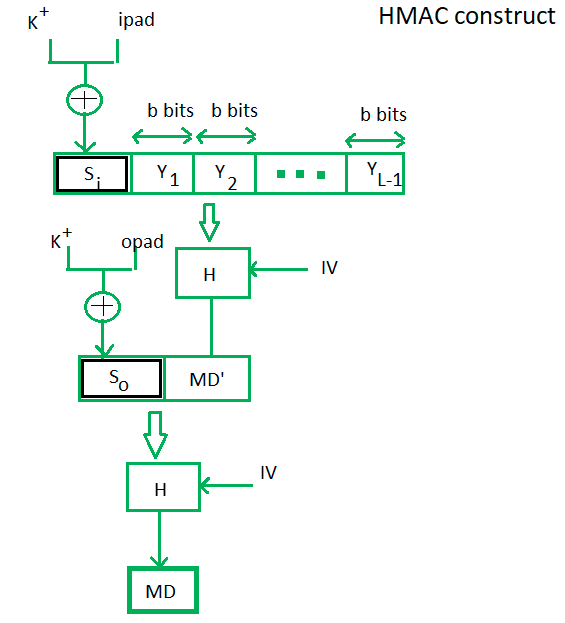
\includegraphics[width=13cm, height=13cm]{Sections/Images/Hash.png}
\end{center}

\newpage
\subsubsection{\textbf{\underline{Le N-MAC}}}

Le \textbf{N-MAC} est une méthode de chiffrement proposé en \textbf{1996} dans un article de \textbf{Mihir Bellare, Ran Conetti et Hugo Krawczyk} dans le but d’améliorer la sécurité du H-MAC, en évitant les attaques basées sue la connaissance partielle de la clé secrète.

\paragraph{Construction du N-MAC}
Le principe de construction du N-MAC est le suivant :
\begin{itemize} 
    \item [\textbullet] On choisit une fonction de hachage H (comme le SHA-256 ou le SHA-512).
    \item [\textbullet] Une clé secrète K.
    \item [\textbullet] On utilise ensuite la fonction de compréssion KDF (key Derivation Function) pour généré les clés K1 et K2 pseudo aléatoirement.
    \item [\textbullet] On calcule S1 = K1 XOR padding interne.
    \item [\textbullet] On calcule S2 = K2 XOR padding externe.
    \item [\textbullet] On calcul le MAC du message M comme :
    MAC (K,K’,M)=H(S1|| H(S2||M) )
\end{itemize}

\paragraph{\textbf{Difficultés}}

Le H-MAC reste tout de même très populaire par rapport au N-MAC car bien que la connaissance partielle de la clé secrète mettrait en danger la sécurité, en pratique, il est très difficile de trouver la \textbf{valeur de la clé secrète interne à partir du MAC}. Même si on connaît le message et la fonction de hachage.
En effet, \textbf{la fonction de hachage est supposée être résistante aux préimages, c’est à dire, qu’il est très difficile de trouver une entrée qui produit une sortie donnée}.Ainsi, pour trouver la clé interne K’, il faudrait résourdre \textbf{l’équation H(K’||M) = MAC}, ce qui est considéré comme infaisable avec les fonctions de Hachage actuelles.De plus, le fait que le N-MAC utilise 2 clés complique la gestion la gestion et la distribution des clés entre les communiquant.

\newpage


\subsection{\textbf{\underline{METHODES DE CONSTRUCTION A BASE DES CODES CORRECTEURS D'ERREURS}}}


Dans le domaine des codes d'authentification de message (MAC), il existe des constructions basées sur des codes correcteurs d'erreurs, technique de codage basee sur la redondance  qui permet non seulement de vérifier l'intégrité des données, mais également de détecter et corriger les éventuelles erreurs de transmission.Les codes correcteurs ont ete invente par Richard Hamming en 1947.Deux constructions couramment utilisées dans les MAC sont le U-MAC et le V-MAC

\subsubsection{\textbf{\underline{ U-MAC (Universal Message Authentication Code)}}}

\textbf{U-MAC} est une construction basée sur les codes correcteurs d'erreurs qui offre à la fois \textbf{l'authentification et la correction d'erreurs}. Il utilise un code correcteur d'erreurs linéaire pour détecter et corriger les erreurs de transmission. Les codes correcteurs d'erreurs linéaires les plus 
couramment utilisés dans le U-MAC sont le \textbf{code de Hamming et le code de Reed-Solomon}.

Voici une description plus détaillée des étapes du U-MAC :
\begin{itemize}[label=$\cdot$]
    \item \textbf{Division du message en blocs :} Le message à authentifier est divisé en blocs de taille fixe. Chaque bloc peut contenir un certain nombre de bits, par exemple 512 bits.
    \item \textbf{Encodage des blocs :} Chaque bloc est encodé à l'aide d'un code correcteur d'erreurs linéaire. L'encodage ajoute des bits de redondance au bloc, ce qui permet de détecter et de corriger les erreurs. Le choix du code correcteur d'erreurs dépend des caractéristiques spécifiques de l'application, telles que le niveau d'erreur attendu et la capacité de correction requise.
    \item \textbf{Génération du MAC :} Une fois les blocs encodés, un MAC est généré pour chaque bloc en utilisant une fonction de hachage cryptographique, telle que SHA-256. Le MAC est calculé sur le bloc encodé, ainsi que sur un numéro de séquence et une clé secrète partagée entre l'expéditeur et le destinataire. Le numéro de séquence est utilisé pour éviter les attaques de rejeu, où un attaquant tente de réutiliser des messages précédemment authentifiés.
    \item \textbf{Transmission des blocs encodés et des MAC }: Les blocs encodés sont transmis avec leurs MAC correspondants. Le destinataire reçoit les blocs encodés et les MAC associés.
    \item \textbf{Vérification du MAC et décodage des blocs :} Le destinataire vérifie l'intégrité des données en recalculant le MAC pour chaque bloc reçu et en le comparant avec le MAC reçu. Si les MAC correspondent, cela indique que le bloc n'a pas été altéré. Ensuite, le destinataire décode les blocs encodés pour récupérer le message d'origine.
    \item \textbf{Correction des erreurs :} Si des erreurs sont détectées dans un bloc, le destinataire utilise les bits de redondance ajoutés lors de l'encodage pour corriger les erreurs. Cela garantit que le message d'origine est récupéré correctement.Le U-MAC offre une combinaison de fonctionnalités d'authentification, de détection et de correction d'erreurs, ce qui en fait une construction robuste pour les applications nécessitant une transmission fiable des données.
\end{itemize} 
\newpage

\subsubsection{\textbf{\underline{Le V-MAC}}}

Le \textbf{V-MAC} est une autre construction basée sur les codes correcteurs d'erreurs, mais avec la particularité de prendre en charge des messages de longueur variable. Contrairement au U-MAC, qui travaille avec des blocs de taille fixe, le V-MAC \textbf{permet d'authentifier des messages de longueur variable, ce qui le rend plus flexible dans certains scénarios.} Il a ete invente par Ted Krovertz et Philip Rogaway


Le V-MAC offre une flexibilité supplémentaire par rapport au U-MAC en \textbf{permettant l'authentification de messages de longueur variable.} Cela peut être utile dans des scénarios où la taille des messages peut varier considérablement, tels que \textbf{les communications en temps réel ou les transferts de fichiers.}\\

Les constructions basées sur les codes correcteurs d'erreurs, comme le U-MAC et le V-MAC, offrent des fonctionnalités d'authentification, de détection et de correction d'erreurs pour assurer l'intégrité des données lors de leur transmission. Ces constructions combinent des codes correcteurs d'erreurs avec des fonctions de hachage cryptographique et des clés secrètes partagées pour garantir la fiabilité des échanges de données. Le choix entre le U-MAC et le V-MAC dépend des exigences spécifiques de l'application et de la nature des messages à authentifier.


\subsection{\textbf{\underline{Référence de cette partie}}}
\begin{center}
    \cite{frwiki:208453934}\\
    \cite{fouque:des-aes}\\
    \cite{frwiki:202365614}\\
    \cite{image:cbc-mac}\\
    \cite{wiki:hash_function}\\
    \cite{okta:hmac}\\
    \cite{okta:umac}\\
    \cite{geeksfg}\\
    \cite{wiki:hmac}\\
    \cite{wiki:umac}\\
    \cite{ionos:hash_function}\\
    \cite{bellare1996new}\\
    \cite{contini2006forgery}\\
    \cite{dodis2012message}
    
\end{center}
\section{\textbf{\underline{UTILISATION DES MAC}}}

Les messages d'authentification par code (MAC) sont largement utilisés dans divers domaines pour garantir la sécurité des communications et protéger les données sensibles. Ils offrent une protection essentielle contre les attaques d'altération et d'usurpation. Nous allons donner quelques exemples d'utilisation du MAC.
\subsection{\textbf{\underline{SECURISATION DES COMMUNICATIONS RESEAUX}}}
Dans cette partie nous aurons principalement deux utilisations du MAC.
\begin{itemize}[label=$\cdot$]
    \item \textbf{\-Protocole des securites reseaux}: les MAC sont utilisés dans des protocoles tels que IPsec pour assurer l'authentification et l'intégrité des paquets de données échangés sur un réseau. En ajoutant un MAC aux paquets, il est possible de vérifier si les données n'ont pas été modifiées en transit.
    \item \textbf{\-Authentification des messages dans les protocoles de securite}: des protocoles de communication tels que TLS/SSL utilisent des MAC pour vérifier l'authenticité et l'intégrité des messages échangés entre les serveurs et les clients. Cela garantit que les données ne sont pas altérées et qu'elles proviennent bien de la source attendue.

\end{itemize}

\subsection{\textbf{\underline{PROTECTION DES DONNEES STOCKEES}}}

\begin{itemize}[label=$\cdot$]
    \item \textbf{\-Authentification des fichiers et des données sensibles} :les MAC sont utilisés pour vérifier l'intégrité des fichiers et des données stockées. En calculant le MAC d'un fichier, il est possible de s'assurer qu'il n'a pas été modifié depuis sa création ou sa dernière vérification.
    \item \textbf{\-Vérification de l'intégrité des sauvegardes}:lors de la création de sauvegardes de données, les MAC sont souvent utilisés pour vérifier l'intégrité des sauvegardes. Cela permet de détecter toute altération ou corruption des données lors de leur restauration.
\end{itemize}

\subsection{\textbf{\underline{AUTHENTIFICATION DES UTILISATEURS}}}

Le MAC permet egalement d'authentifier les differents utilisateurs sur le reseau.

\begin{itemize}[label=$\cdot$]
        \item \textbf{Mécanismes d'authentification forte}:les MAC sont utilisés dans des mécanismes d'authentification forte tels que HMAC-based One-Time Passwords (HOTP). Ces mécanismes génèrent des codes d'authentification uniques à chaque utilisation, basés sur un secret partagé et un compteur. Les MAC sont utilisés pour valider ces codes d'authentification.
        \item \textbf{Protection des mots de passe} :les MAC sont utilisés pour protéger les mots de passe stockés dans les bases de données. Lorsqu'un utilisateur saisit un mot de passe, son MAC est calculé et comparé avec celui stocké dans la base de données. Cela permet de vérifier l'authenticité du mot de passe sans stocker le mot de passe lui-même.

\end{itemize}
\newpage

\subsection{\textbf{\underline{Référence de cette partie}}}
\begin{center}
    \cite{cini2021updatable}\\
    \cite{athmani2010protocole}\\
    \cite{dierks2008transport}\\
    \cite{mckusick2015design}\\
    \cite{krawczyk2010cryptographic}\\
    \cite{turner2008keyed}\\
    \cite{vazquez2021pakemail}\\
\end{center}
\section{\textbf{\underline{AVANTAGES DES MAC}}}

Nous allons donner quelques avantages cles des MAC:

\begin{enumerate}
    \item \textbf{Intégrité des données}:les MAC garantissent l'intégrité des données échangées. En calculant un MAC pour un message, il est possible de détecter si les données ont été altérées pendant leur transmission. Si le MAC calculé ne correspond pas au MAC reçu, cela indique qu'une altération a eu lieu.
    \item \textbf{Authentification des sources}:les MAC fournissent une authentification des sources des messages. En utilisant une clé secrète partagée pour générer le MAC, le destinataire peut vérifier que le message provient d'une source authentique. Cela protège contre les attaques d'usurpation où un attaquant tente de se faire passer pour une entité légitime.
    \item \textbf{Simplicité et efficacité}:les MAC sont relativement simples à implémenter et à vérifier. Les algorithmes de MAC couramment utilisés, tels que HMAC (HMAC-MD5, HMAC-SHA1, HMAC-SHA256, etc.), sont largement disponibles et bien documentés. De plus, le processus de vérification du MAC est efficace et ne nécessite pas de déchiffrer le contenu du message.
    \item \textbf{Non-répudiation (dans certains cas)}:dans certains scénarios, les MAC peuvent être utilisés pour fournir une preuve de l'origine d'un message, ce qui permet de résoudre les problèmes de non-répudiation. Si une clé secrète est associée à une entité spécifique, le MAC peut servir de preuve que cette entité a généré le message.
    \item \textbf{Adaptabilité}:les MAC peuvent être utilisés dans une variété de scénarios et de protocoles, tels que les communications réseau, les protocoles de sécurité, l'authentification des utilisateurs et la protection des données stockées. Ils peuvent être intégrés dans des protocoles existants sans nécessiter de modifications majeures.
    \item \textbf{Résistance aux attaques cryptographiques courantes}:les MAC sont conçus pour résister à diverses attaques cryptographiques, y compris les attaques par force brute, les attaques par collision et les attaques par choix de messages. Les algorithmes de MAC bien conçus offrent un niveau élevé de sécurité contre ces attaques.\\
\end{enumerate}

\subsection{\textbf{\underline{Référence de cette partie}}}
\begin{center}
    \cite{Fortinet}\\
    \cite{bellare1996keying}\\
    \cite{klima2018cryptology}\\
    \cite{paar2009understanding}\\
    \cite{stallings2017principles}\\
    \cite{schneier1995applied}\\
\end{center}
\section{\textbf{\underline{SECURITE DES MAC}}}

\subsection{\textbf{\underline{VULNERABILITES POTENTIELLES DES MAC}}}

Les MAC sont sujets à différentes vulnérabilités potentielles qui peuvent compromettre leur sécurité. Voici quelques-unes des principales vulnérabilités :

\begin{itemize}[label=$\cdot$]
    \item \textbf{Attaques de force brute}:les MAC sont généralement basés sur des fonctions de hachage cryptographique résistantes aux collisions. Cependant, si la fonction de hachage utilisée est vulnérable aux attaques de force brute, un attaquant peut essayer différentes clés secrètes jusqu'à ce qu'il trouve celle qui génère le même MAC que celui observé. Cela peut être prévenu en utilisant des clés suffisamment longues et en choisissant des fonctions de hachage résistantes aux attaques de force brute.
    \item \textbf{Attaques de collision}:les attaques de collision visent à trouver deux messages différents qui génèrent le même MAC. Si un attaquant parvient à générer une collision, il peut substituer un message valide par un autre message ayant le même MAC sans être détecté. Pour prévenir ces attaques, il est essentiel d'utiliser des fonctions de hachage cryptographique résistantes aux collisions, telles que les fonctions de hachage basées sur la famille des algorithmes SHA (Secure Hash Algorithm).
    \item \textbf{Attaques par clé faible}: Si une clé secrète utilisée dans le MAC est faible, par exemple, si elle est facilement devinable ou si elle a une faible entropie, un attaquant peut la déterminer et générer des MAC valides. Il est donc crucial d'utiliser des clés secrètes suffisamment longues et aléatoires.
    \item \textbf{Attaques par canal auxiliaire} : Les MAC peuvent être vulnérables à des attaques par canal auxiliaire, où un attaquant exploite des informations supplémentaires obtenues à partir d'un autre canal pour compromettre la sécurité du MAC. Par exemple, des attaques basées sur la consommation d'énergie ou les temps d'exécution peuvent révéler des informations sur la clé secrète utilisée dans le MAC. La protection contre ces attaques nécessite des contre-mesures spécifiques, telles que l'utilisation de méthodes de masquage ou de contre-mesures matérielles
\end{itemize}

\subsection{\textbf{\underline{TECHNIQUES DE RENFORCEMENT DES MAC}}}

Pour renforcer la sécurité des MAC, plusieurs techniques peuvent être mises en œuvre :

\begin{itemize}[label=$\cdot$]
    \item \textbf{Utilisation de fonctions de hachage cryptographique sécurisées}:les MAC dépendent de fonctions de hachage cryptographique pour générer des valeurs de hachage. Il est important d'utiliser des fonctions de hachage réputées, telles que les variantes de la famille des algorithmes SHA, qui ont été largement étudiées et analysées par la communauté de la cryptographie.
    \item \textbf{Utilisation de clés secrètes fortes}:les clés secrètes utilisées dans les MAC doivent être suffisamment longues et aléatoires pour résister aux attaques par force brute. Il est recommandé d'utiliser des générateurs de nombres aléatoires cryptographiquement sécurisés pour générer les clés.
    \item \textbf{Utilisation de clés différentes pour chaque session} : L'utilisation de clés différentes pour chaque session de communication renforce la sécurité du MAC. Cela empêche un attaquant d'exploiter les informations obtenues à partir d'une session pour compromettre les sessions ultérieures.
    \item \textbf{Utilisation de MAC basés sur des constructions sécurisées} : Il existe des constructions de MAC spécifiques qui ont été prouvées sécurisées contre certaines classes d'attaques. Par exemple, le HMAC (Hash-based Message Authentication Code) est une construction de MAC largement utilisée qui utilise une fonction de hachage cryptographique et une clé secrète pour générer le MAC.
\end{itemize}

\subsection{\textbf{\underline{EVOLUTION DU MAC POUR FAIRE FACE AUX NOUVELLES MENACES}}}

Les MAC évoluent continuellement pour faire face aux nouvelles menaces et aux avancées de la cryptanalyse. Voici quelques développements récents :

\begin{itemize}[label=$\cdot$]
    \item \textbf{MAC basés sur les chiffrements authentifiés}:les constructions de MAC basées sur les chiffrements authentifiés, tels que les modes d'opération AES-GCM (Advanced Encryption Standard - Galois/Counter Mode), offrent à la fois l'authentification et le chiffrement des données. Ces constructions combinent les propriétés de confidentialité et d'intégrité dans un seul mécanisme, ce qui les rend efficaces pour protéger les communications.
    \item \textbf{MAC résistants aux attaques par canal auxiliaire}:les chercheurs travaillent sur le développement de MAC résistants aux attaques par canal auxiliaire. Des techniques telles que le masquage, qui consistent à introduire du bruit aléatoire dans les opérations cryptographiques, sont utilisées pour rendre les MAC moins sensibles aux fuites d'informations par le biais de canaux auxiliaires.
    \item \textbf{MAC résistants aux attaques par collision} : Pour prévenir les attaques par collision, de nouvelles constructions de MAC résistantes aux collisions sont développées. Par exemple, le Poly1305 est un MAC basé sur une fonction de hachage non sécurisée contre les collisions, mais qui est prouvé sûr lorsqu'il est utilisé avec une clé secrète unique.
    \item \textbf{MAC basés sur la cryptographie quantique} : Avec l'avènement de la cryptographie quantique, de nouveaux types de MAC basés sur des primitives quantiques sont étudiés. Ces MAC utilisent des propriétés quantiques, telles que l'intrication quantique, pour garantir la sécurité et la confidentialité des messages.
\end{itemize}

\subsection{\textbf{\underline{Référence de cette partie}}}
\begin{center}
    \cite{bellare2000new}\\
    \cite{dodis2005fuzzy}\\
    \cite{gennaro2004secure}\\
    \cite{bellare1996keying}\\
    \cite{wang2005finding}\\
\end{center}
\section{\textbf{\underline{IMPLEMENTATION DU MAC EN PYTHON}}}

L'implémentation en python de notre thème, entre outre les MACs, concerne un type de MAC en particulier : les CBC-MACs. En effet, elle consiste en le développement d'une mini-plateforme de messagerie simple sur serveur local. En d'autres termes, notre application s'exécute uniquement à partir d'une seule machine. Notons qu'il est toutefois possibles d'en lancer plusieurs instances indépendantes depuis celle-ci. De plus, notre plateforme dispose des options fondamentales y relatives, entre autres :
\begin{itemize}[label=$\cdot$]
    \item Possibilité de se connecter à son compte (si bien entendu il existe déjà) : pour cela, il doit tout simplement entrer son adresse e-mail et son mot de passe, suite à quoi il lui suffit de cliquer sur 'connexion' pour se connecter. Suite à cela, une boîte de dialogue 'Connexion réussie à l'adresse ...' s'affiche et l'utilisateur peut choisir d'envoyer un message ou de consulter les messages qu'il a reçu.
    \item Possibilité de créer un compte : ceci consiste, pour l'utilisateur, à entrer des informations personnelles comme son nom et son prénom, sa date de naissance, son numéro de téléphone, et de choisir son mot de passe (qui doit absolument être non vide). Une fois ces informations remplies, il peut cliquer sur 'générer adresse' pour voir l'adresse qui lui sera attribuée. Il peut ensuite choisir de créer un compte, ce qui le fera se 'connecter' à son compte nouvellement créé. Suite à cela, une boîte de dialogue 'Connexion réussie à l'adresse ...' s'affiche et l'utilisateur peut choisir d'envoyer un message ou de consulter les messages qu'il a reçu.
    \item Possibilité d'envoyer un message : pour le faire, une fois connecté, l'utilisateur n'a plus qu'à choisir l'option 'Envoyer un message'. Aussitôt choisie, une nouvelle fenêtre s'affiche, précédée de la disparition de la fenêtre précédente. Cette fenêtre demande obligatoirement d'entrer l'adresse du destinataire (si on la laisse vide et qu'on clique sur 'envoyer', une boîte de dialogue signale "adresse de destinataire vide") et celle-ci doit être correcte (si on entre une adresse inexistante et qu'on clique sur 'envoyer', une boîte de dialogue signale "adresse de destinataire incorrecte"). A part l'adresse du destinataire, il est possible d'entrer un message et/ou un objet. Le message ne doit pas être vide (si il est malgré tout vide, le MAC y correspondant sera vide). Si les conditions précédentes sont réunies une boîte de dialogue 'votre message a été correctement envoyé' s'affiche).
    \item Possibilité de consulter les messages reçus : si l'on clique sur 'consulter les messages reçus', le programme parcourt d'abord une première fois tous les messages reçus (au passage, par la boîte de dialogue 'Ce message n'est pas authentique, il ne sera pas affiché', il signale tous les messages non authentiques/intègres). Il s'arrête sur le dernier message reçu par l'utilisateur. Celui-ci a ensuite la possibilité de consulter un à un les messages qu'il a reçu en naviguant dans sa boîte de réception à l'aide de 'Previous' et de 'Next'. Ceux-ci deviennent blancs s'il n'y a plus de messages respectivement avant celui sélectionné et/ou après. Dans le cas contraire ils sont verts. Si dans la navigation, on essaie de consulter un message qui n'est pas authentique, le programme affiche une boîte de dialogue 'Ce message n'est pas authentique, il ne sera pas afiifiché' et celui-ci n'est effectivement pas affiché. Pour chaque message reçu, le programme affiche l'objet et l'adresse de l'émetteur. et si celui-ci est authentique, il affiche aussi son contenu dans une zone de texte situé en plein milieu de la page.
\end{itemize}

Il est à noter que notre programme ne permet pas d'envoyer de confirmations de lectures, ni la date d'envoi des messages. Cependant, il vérifie l'ordre des messages reçus à travers le MAC. En effet, les MACs sont générés diffèrent en fonction de la position du message dans la boîte de réception du destinataire.

Lors de l'envoi, le MAC est calculé au moyen d'un algorithme de chiffrement CBC et la clé secrète qu'un couple (émetteur-destinataire) a en commun est calculée par le programme afin d'éviter qu'elle soit stockée en mémoire. Son algorithme de calcul est complexe et difficile à conjecturer. Elle varie en fonction de l'émetteur et du destinataire (en fait cette clé est différente même pour peu que l'on inverse l'émetteur et le destinataire). Le vecteur d'initialisation du CBC est basé sur un générateur pseudo aléatoire qui dépend de la position du message dans la boîte de réception du message. 
L'intérêt du dispositif est qu'il permet de vérifier l'ordre d'arrivée des messages afin de vérifier un potentiel réenvoi d'un même message par un hacker 'lambda'.

En parallèle, nous avons développé une plateforme qui permet une modification quelconque d'un message dans la boîte de réception d'un utilisateur dont l'adresse a été préalablement entrée. Ceci va nous permettre d'illustrer l'efficacité des MACs dans la vérification de l'intégrité des MACs. Aussi, pendant l'illustration, nous allons vous montrer l'intérêt du générateur pseudo-aléatoire en dupliquant (par exemple) un message et son MAC.

Au terme de notre illustration, nous espérons vous avoir définitivement convaincu sur l'importance des MACs et nous souhaitons que vous serez fascinés par les MACs, fascination qui d'ailleurs nous a poussés a créer notre propre fonction de génération de clés.

\newpage
\subsection{\textbf{\underline{Key Generation Function}}}

\begin{Pythoncode}[numbers=left, caption={Python Code}]
def genPseudoAl(ke : str, i : int):
    s = ""
    l = TAILLE // i
    l %= TAILLE
    m = 1
    while len(s) != TAILLE:
        s += ke[l]
        m += 1
        l += TAILLE // m
        l %= TAILLE
    return s
\end{Pythoncode}

\subsection{\textbf{\underline{CBC MAC Function}}}

\begin{Pythoncode}[numbers=left, caption={Python Code}]
def CBC(st : str, ke : str, a : int):#cryptage CBC
    ke = genPseudoAl(ke, a)
    if len(st) % TAILLE != 0:
        while len(st) % TAILLE != 0:
            st = "0"+st
    for i in range(len(st) // TAILLE):
        x = st[TAILLE*i:TAILLE*(i+1)]
        k = ""
        for j in range(len(x)):
            if x[j] == ke[j]:
                k += "0"
            else:
                k += "1"
        a += 1
        ke = genPseudoAl(k , a)
    if(len(st) != 0):
        return(ke)
    else:
        return("")
    pass
\end{Pythoncode}
\newpage

\begin{Pythoncode}[numbers=left, caption={Python Code}]
def key(senderadr : str, receiveradr : str):#générateur de clés
    s = ""
    senderadr = senderadr[:-12]
    receiveradr = receiveradr[:-12]
    if len(senderadr) > len(receiveradr):
        for i in range(len(receiveradr)):
            s += senderadr[i]
            s += receiveradr[i]
        s += senderadr[len(receiveradr):]
    elif len(receiveradr) > len(senderadr):
        for i in range(len(senderadr)):
            s += senderadr[i]
            s += receiveradr[i]
        s += receiveradr[len(senderadr):]
    else:
        for i in range(len(senderadr)):
            s += senderadr[i]
            s += receiveradr[i]
    k1 = ""
    for i in s[0:]:
        k1 += str(bin(ord(i)))[2:]
    k = ""
    if len(k1) < TAILLE:
        k = k1
        j = 0
        i = 0
        while len(k) < TAILLE:
            k += k1[i]
            j += 1
            i += len(k1) // j
            i %= len(k1)
    else:
        k = k1[:TAILLE]
    return(k)#longeur TAILLE
    pass
\end{Pythoncode}
\newpage

\subsection{\textbf{\underline{Tkinter Interface}}}

\begin{Pythoncode}[numbers=left, caption={Python Code}]
def sendmessage(adr : str):#cette fonction permet d'envoyer des messages depuis l'adresse spécifiée en paramètre
    r = Tk()
    ad = StringVar()
    obj = StringVar()
    def test():
        try:
            if ad.get() != adr:
                os.chdir(ad.get())
                bt = True
                i = 0
                tmp = None
                while bt:
                    try:
                        tmp = open(str(i)+".msg", "r")
                        tmp.close()
                        i = i + 1
                    except FileNotFoundError:
                        bt = False
                s = mes.get("1.0", END)
                s1 = s[0:-1]
                tmp = open(str(i)+".msg", "w")
                tmp.write(s1)
                tmp.close()
                tmp = open("sender"+str(i)+".snd", "w")
                tmp.write(adr)
                tmp.close()
                tmp = open("object"+str(i)+".obj", "w")
                tmp.write(obj.get())
                tmp.close()
                tmp = open("MAC"+str(i)+".mac", "w")
                s = ""
                for j in s1:
                    s += str(bin(ord(j)))[2:]
                MAC = CBC(s, key(adr, ad.get()), i + 1)
                tmp.write(MAC)
                tmp.close()
                os.chdir("..")
                r.destroy()
                messagebox.askokcancel("Envoyé", "Votre message a été envoyé ...")
                return
            else:
                messagebox.askokcancel("Erreur", "Vous ne pouvez pas vous écrire ...")
        except OSError:
            messagebox.askokcancel("Erreur", "Adresse de destinataire incorrecte, veuillez recommencer")
        pass
    r.geometry("600x500+300+10")
    r.title("Send a Message ...")
    r.resizable(False, False)
    c = Canvas(r, bg="#fef1e1")
    c.pack(expand=YES, fill=BOTH)
    Label(c, text="Send to :", bg="#fef1e1", font=("Times New Roman", 14), fg="black").place(x=10, y=15)
    Entry(c, textvariable=ad, font=("Times New Roman", 14), fg="black").place(x=100, y=15, width=400)
    Label(c, text="Object :", bg="#fef1e1", font=("Times New Roman", 14), fg="black").place(x=10, y=60)
    Entry(c, textvariable=obj, font=("Times New Roman", 14), fg="black").place(x=100, y=60, width=400)
    mes = scrolledtext.ScrolledText(c, font=("Times New Roman", 14), fg="black")
    mes.place(x=15, y=110, width=565, height=330)
    ad.set("")
    obj.set("")
    Button(c, command=test, bg="#058747", text="Send Message", font=("Times New Roman", 14), fg="white").place(x=15, y=450)
    r.mainloop()
    l = logged(adr)
    l.activate()
    pass
\end{Pythoncode}

\newpage
\begin{Pythoncode}[numbers=left, caption={Python Code}]
class logged :#c'est la classe qui permet l'interaction entre 
    root = None
    panel = None
    lirem = None
    sendm = None
    adr = None
    read = True

    def readmessages(self):
        os.chdir(self.adr)
        self.root.destroy()
        view(self.adr)

        pass

    def sendmessages(self):
        self.root.destroy()
        sendmessage(self.adr)

        pass

    def __init__(self, adr : str) -> None:
        self.adr = adr
        self.root = Tk()

        self.root.geometry("320x200+300+200")
        self.root.title(adr)
        self.root.resizable(False, False)

        self.panel = Canvas(self.root, bg="#fef1e1")
        self.panel.pack(expand=YES, fill=BOTH)

        Button(self.panel, text="Write Messages", command=self.sendmessages, font=("Times New Roman", 18), bg="#058747", fg="white").place(x=70, y=40)
        
        Button(self.panel, text="Read Messages ", command=self.readmessages, font=("Times New Roman", 18), bg="#058747", fg="white").place(x=70, y=100)
        
        pass

    def activate(self):
        self.root.mainloop()
        pass
\end{Pythoncode}
\newpage

\begin{Pythoncode}[numbers=left, caption={Python Code}]
#classe qui peut créer les nouveaux utilisateurs
class newUser :
    x = None
    x = open("i", "r")
    i = int(x.readline())
    x.close()
    i += 1
    root = None
    panel = None
    noms = None
    daten = None
    nom = None
    datenaiss = None
    password = None
    paw = None
    tele =  None
    tel = None
    visible = False
    voir = None
    adr = None
    log = None
    def adresse(self):
        x = open("i", "r")
        self.i = int(x.readline())
        x.close()
        self.i += 1
        self.adr.config(text="ADRESSE : "+self.nom.get().lower().replace(" ","")+str(self.i)+"@macmail.com")
        pass
    def connection(self):
        if self.paw.get() == "" or self.paw.get().split() == []:
            messagebox.askokcancel("Erreur", "Pas de mot de passe ...")
        else:
            self.adresse()
            s = str(self.adr.__getitem__("text"))
            s1 = ""
            for i in range(len(s)):
                if i < 10:
                    pass
                else:
                    s1+=s[i]
            x = open("adresses", "r")
            s = ""
            for i in x.readlines():
                s += i
            x.close()
            x = open("adresses", "w")
            x.write(s+s1+" "+self.paw.get()+"\n")
            x.close()
            self.root.destroy()
            messagebox.askokcancel("Votre adresse", "Votre adresse est "+s1)
            self.log = logged(s1)
            x = open("i", "w")
            x.write(str(self.i))
            x.close()
            os.mkdir(s1)
            self.log.activate()
        pass
    def Voir(self):
        #cette fonction permet de switcher entre les modes visible et non visible du champ de mot de passe
        if self.visible == False:
            self.password.config(show="")
            self.voir.config(text="Hide", bg="grey", fg="#ff8e01")
            self.visible = True
        else:
            self.password.config(show="*")
            self.voir.config(text="Show",bg="white", fg="#ff8e01")
            self.visible = False
        pass
    def __init__(self) -> None:
        self.root = Tk()
        self.nom = StringVar()
        self.paw = StringVar()
        self.tel = StringVar()
        self.daten = StringVar()
        self.root.geometry("600x450+180+50")
        self.root.title("Nouveau Compte")
        self.root.resizable(False, False)
        self.panel = Canvas(self.root, bg= "#fef1e1")
        self.panel.pack(expand=YES, fill=BOTH) 
        Label(self.panel, text="Create a new account",font=("Georgia", 30),bg="white", fg="#ff8e01").place(x=40, y=3)
        self.panel.create_rectangle(0, 65, 450, 450,outline="grey", width=0, fill="white")
        self.panel.create_line(0,65,450,65, width=1, fill="grey")
        self.panel.create_line(450,0,450,450, width=1, fill="grey")
        self.panel.create_rectangle(0, 0, 450, 65,outline="grey", width=0, fill="white")
        Label(self.panel, text="Name:", font=("Times New Roman", 14), fg="black", bg="white").place(x=5, y=75, height=30)
        self.noms = Entry(self.panel, textvariable=self.nom, fg="black", bg="#fef1e1", font=("Times New Roman", 12))
        self.noms.place(x=60, y=75, width=365, height=30)
        Label(self.panel, text="Date of Birth:", font=("Times New Roman", 14), fg="black", bg="white").place(x=5, y=120, height=30)
        self.datenaiss = Entry(self.panel, textvariable=self.daten, fg="black", bg="#fef1e1", font=("Times New Roman", 12))
        self.datenaiss.place(x=110, y=120, width=315, height=30)
        Label(self.panel, text="Phone number:", font=("Times New Roman", 14), fg="black", bg="white").place(x=5, y=165, height=30)
        self.tele = Entry(self.panel, textvariable=self.tel, fg="black", bg="#fef1e1", font=("Times New Roman", 12))
        self.tele.place(x=125, y=165, width=300, height=30)
        Label(self.panel, text="Password:", font=("Times New Roman", 14), fg="black", bg="white").place(x=5, y=210, height=30)
        self.password = Entry(self.panel, textvariable=self.paw, fg="black", bg="#fef1e1", font=("Times New Roman", 12), show="*")
        self.password.place(x=90, y=210, width=280, height=30)
        self.voir = Button(self.panel, text="Show",bg="white", fg="#ff8e01", command=self.Voir, font=("Times New Roman", 14))
        self.voir.place(x=370, y=210, height=30)
        self.adr = Label(self.panel, text="Address : ", font=("Times New Roman", 14), fg="black", bg="white")
        self.adr.place(x=10, y=270, height=35)
        self.adresse()
        Button(self.panel, text="Generate Address", command=self.adresse, font=("Times New Roman", 14), bg="#058747", fg="white").place(x=300, y=315)
        Label(self.panel, text="Remember your address", font=("Times New Roman", 11), bg="White", fg="black").place(x=20, y=310)
        Label(self.panel, text="you'll need it to login to your account !", font=("Times New Roman", 11), bg="White", fg="black").place(x=20, y=335)
        Button(self.panel, text="Create Account", command=self.connection, font=("Times New Roman", 14), bg="#058747", fg="white").place(x=140, y=380, height=40)
        pass
    def activate(self):
        self.root.mainloop()
        pass
\end{Pythoncode}
\newpage

\begin{Pythoncode}[numbers=left, caption={Python Code}]
#classe qui permet de se connecter (c'est la première classe qui est créée en mémoire)
class connection :
    #quelques variables utiles
    root = None
    panel = None
    adresse = None
    adr = None
    password = None
    paw = None
    visible = False
    voir = None
    newu = None
    log = None
    line = None

    def Voir(self):
        #cette fonction permet de switcher entre les modes visible et non visible du champ de mot de passe
        if self.visible == False:
            self.password.config(show="")
            self.voir.config(text=" Hide ", bg="grey", fg="#ff8e01")
            self.visible = True
        else:
            self.password.config(show="*")
            self.voir.config(text="Show",bg="white", fg="#ff8e01")
            self.visible = False

        pass

    def connect(self):
        #cette fonction permet d'engendrer le processus de connexion à la plateforme de messagerie
        x = open("adresses", "r")
        b = False
        for i in x.readlines():
            """ k = i """
            s1 = ''
            s2 = ''
            for j in range(len(i)):
                if i[j] != ' ':
                    s1 += i[j]
                else:
                    s2 = i[j+1:-1]
                    break
            """ for j in range(2, len(k)):
                k[1] += " "+k[j] """
            if s1 == self.adr.get() and s2 == self.paw.get():
                b = True
                break

        x.close()

        if b:
            s = self.adr.get()
            self.root.destroy()
            messagebox.askokcancel("Connexion", "Connexion réussie à l'adresse "+s)
            self.log = logged(s)
            self.log.activate()
        else:
            messagebox.askokcancel("Erreur", "Identifiant ou mot de passe incorrect ...")

        pass

    def newuser(self):
        #cette fonction permet de lancer la classe newUser au cas où l'utilisateur le souhaite
        self.root.destroy()
        self.newu = newUser()
        self.newu.activate()

        pass

    def __init__(self) -> None:
        #ici on initialise l'interface graphique
        self.root = Tk()
        self.root.geometry("1000x600+20+30")
        self.adr = StringVar()
        self.paw = StringVar()
        self.root.title("Connexion")
        self.root.resizable(False, False)

        self.panel = Canvas(self.root, bg= "#fef1e1")
        self.panel.pack(expand=YES, fill=BOTH)
        
        self.panel.create_rectangle(0, 130, 750, 600,outline="grey", width=0, fill="white")
        
        self.panel.create_line(0,130,750,130, width=1, fill="grey")
        self.panel.create_line(750,0,750,600, width=1, fill="grey")
        self.panel.create_rectangle(0, 0, 750, 130,outline="grey", width=0, fill="white")

        Label(self.panel, text="Sign In",font=("Georgia", 55),bg="white", fg="#ff8e01").place(x=200, y=3)
        Label(self.panel, text="Create a new account",font=("Georgia", 10),bg="white", fg="#ff8e01").place(x=250, y=100)
        
        Label(self.panel, text="Address:", font=("Times New Roman", 28), fg="black", bg="white").place(x=5, y=185, height=30)

        self.adresse = Entry(self.panel, textvariable=self.adr, fg="black", bg="#fef1e1", font=("Times New Roman", 28))
        self.adresse.place(x=150, y=180, width=490, height=45)

        Label(self.panel, text="Password:", font=("Times New Roman", 28), fg="black", bg="white").place(x=5, y=275, height=30)
        
        self.password = Entry(self.panel, textvariable=self.paw, fg="black", bg="#fef1e1", font=("Times New Roman", 28), show="*")
        self.password.place(x=165, y=270, width=465, height=45)

        self.voir = Button(self.panel, text="Show",bg="white", fg="#ff8e01", command=self.Voir, font=("Times New Roman", 28))
        self.voir.place(x=630, y=270, height=45)
       
        Button(self.panel, text="Login", command=self.connect, font=("Times New Roman", 28), bg="#058747").place(x=260, y=350, height=45)

        Label(self.panel, text="You don't have an account yet?",font=("Times New Roman", 20), bg="white").place(x=15, y=450)
        Label(self.panel, text="Sign Up Now !",font=("Times New Roman", 28), bg="white").place(x=15, y=500, height=45)

        
        Button(self.panel, text="Get Started", command=self.newuser, font=("Times New Roman", 28),bg="white", fg="#ff8e01").place(x=260, y=500, height=45)
        
        pass

    def activate(self):
        #cette fonction permet de lancer effectivement l'application
        self.root.mainloop()
        pass
\end{Pythoncode}
\begin{center}\textbf{\underline{CONCLUSION}}
\end{center}

Nous sommes maintenant rendus au terme de notre 
exposé.Tout au long de celui-ci, il était question pour nous de vulgariser la notion de Message Authentification Code. En effet, tout au long de notre présentation, nous vous avons tour à tour présenté :leur définition;leur fonctionnement;leurs méthodes de construction;la façon dont on peut les utiliser;leurs avantages;leurs failles;la manière dont ils ont évolués pour s'adapter aux attaques.De ce qui précède, nous pouvons conclure que les MACs représentent un outil essentiel pour l'épanouissement individuel de tout un chacun au sein de sa vie sociale sur Internet. Nous devons cependant ajouter qu'ils ont besoin de constamment évoluer pour faire fâce à de plus en plus d' attaques. Pour ces raisons, il est essentiel, pour l'ingénieur informaticien de s'y intéresser et ce dans l'optique de garantir l'authenticité et l'intégrité des données circulant sur le web en général, et celle des messages en particulier.\\
\\
\section{\textbf{\underline{EXERCICES CONCERNANT LE MAC}}}

Cette partie comporte une serie de questions permettant de nous rassurer que vous avez bien compris les MACs. Vous constituerez des équipes de 3 personnes pour y répondre. 

%----------------------Exo 1-----------------------------
\subsection{\textbf{\underline{Exercice 1}}} 
\label{Exo 1}

\begin{enumerate}
    \item [\textbf{Q01}] Laquelle/Lesquelles de ces affirmations est erronnée :
    \begin{itemize}
        \item [i.] Les MACs permettent de garantir l'intégrité des messages
        \item [ii.] Les MACs permettent de garantir la confidentialité des messages
        \item [iii.] Les MACs permettent de garnatir la non répudiation
        \item [iv.] Les MACs permettent de garantir la chronologie des messages
    \end{itemize}
    
    \item [\textbf{Q02}:] Comment fonctionnent les HMACs ?
    
    \item [\textbf{Q03}:] Comment fonctionnent les NMACs ?

    \item [\textbf{Q04}:] Comment fonctionnent les CMACs ?
    
    \item [\textbf{Q05}:] Quelles sont les limites de HMACs ?
    
    \item [\textbf{Q06}:] Quelles sont les limites des CBC-MACs ?
    
    \item [\textbf{Q07}:] Comment faire pour garantir la chronologie des messages quand on utilise les MACs ?
    
    \item [\textbf{Q08}:] Comment renforcer les CBCMACs ?
    
    \item [\textbf{Q09}:] Quels sont les avantages des HMACs ?
    
    \item [\textbf{Q10}:] Comment renforcer les HMACs ?
    
    \item [\textbf{Q11}:] Pour les MACs à chiffrement par blocs, quels sont les critères d'un bon générateur pseudo-aléatoire de clés ?
    
    \item [\textbf{Q12}:] En utilisant uniquement les MACs, peut-on garantir la réception de tous les messages ?
    
    \item [\textbf{Q13}:] Quelles améliorations proposez vous pour les MACs ?\\
\end{enumerate}

\par Pour aller à la \nameref{C_Exo 1}

%----------------------------------------------------------

%----------------------Exo 2-------------------------------
\subsection{\textbf{\underline{Exercice 2}}}
\label{Exo 2}

Soit H une fonction de hachage qui prend en entrée un message m de longueur arbitraire et qui renvoie une sortie de longueur fixe n bits.

On définit le MAC suivant : pour un message m et une clé secrète k de longueur n bits, on calcule MAC(m,k)=H(m$\parallel$k), où $\parallel$ désigne la concaténation de chaînes de bits.
\begin{enumerate}
    \item [\textbf{1.}] Montrer que ce MAC n’est pas sûr, c’est-à-dire qu’un adversaire peut forger un message valide avec une probabilité non négligeable, sans connaître la clé secrète k.
    \item [\textbf{2.}] Proposer une modification du MAC pour le rendre plus sûr, en utilisant la même fonction de hachage H et la même clé secrète k.
\end{enumerate}

\subsubsection{\textbf{\underline{References de cet exercice}}}
Jean-Guillaume Dumas,Jean-louis Roch,Eric Tannier,Sebastien Varette,"Theorie Des Codes" P.185\\

\par Pour aller à la \nameref{C_Exo 2}

%-----------------------------------------------------------

%--------------------Exo 3-----------------------------------
\subsection{\textbf{\underline{Exercice 3}}}
\label{Exo 3}

\textbf{\underline{NB:}}Pour cette exercice, s'il vous plait veuillez ajouter les zeros au debut de la chaine 

Voici le code python d'un générateur pseudo aléatoire :

\begin{Pythoncode}[numbers=left, caption={Python Code}]
def genPseudoAl(ke : str, i : int):
    s = ""
    l = TAILLE // i
    l %= TAILLE
    m = 1
    while len(s) != TAILLE:
        s += ke[l]
        m += 1
        l += TAILLE // m
        l %= TAILLE
    return s
\end{Pythoncode}


Supposons 	qu'une 	clé 	secrète 	soit 	: 	k 	= 
'101010010101001110101010010110101011101001011001010
111010010101010101111001111011101111110110011011010
101001101011001110111100'

Considérons les messages suivants : "Bonjour, comment vas tu", "Salut, à bientôt", "Rendez-vous ce soir à 20h", "J'ai adoré cette sortie", "J'aime coder en python", "Je déteste le langage PHP", "Tu es un ange", "Toi \& moi on est pareils"  sachant que l'algorithme de calcul de MAC convertit les lettres et les chiffres (les caractères spéciaux aussi) en binaire suivant la norme ASCII à 7 chiffres, calaculez le MAC de chaque message (utilisez la convention CBC MAC). 

Vous utiliserez le générateur pour calculer le vecteur d'initialisation d'abord (en mettant i à 1) puis vous l'utiliserez pour trouver chaque vecteur de chiffrement intermédiaire (à chaque nouveau vecteur on incrémente i avant de lancer le générateur).\\

\par Pour aller à la \nameref{C_Exo 3}
%----------------------------------------------------------

%-----------------------Exo 4------------------------------
\subsection{\textbf{\underline{Exercice 4}}}
\label{Exo 4}

Supposons que vous ayez une clé secrète de 8 chiffres (par exemple, 12345678) et un message de texte brut (par exemple, "Hello, world!"). Votre tâche est de générer un MAC en utilisant l'algorithme HMAC-SHA256.

\begin{enumerate}
    \item Convertissez la clé secrète en une séquence de chiffres hexadécimaux (base 16). Par exemple, 12345678 devient 3132333435363738.
    
    \item Concaténez la clé secrète convertie avec le message de texte brut. Par exemple, si le message est "Hello, world!", la concaténation serait 3132333435363738Hello, world!

    \item Utilisez une fonction de hachage SHA256 pour calculer le haché (digest) de la concaténation obtenue.

    \item Le haché obtenu est le MAC généré.\\
\end{enumerate}

\par Pour aller à la \nameref{C_Exo 4}
%---------------------------------------------------------

\section{\textbf{\underline{CORRECTION DES EXERCICES}}}
%----------------------Exo 1-----------------------------
\subsection{\textbf{\underline{Correction de l'exercice 1}}}\label{C_Exo 1}

\begin{enumerate}
    \item [\textbf{Q01}] La deuxième, troisième et la quatrième affirmation est erronée.\\

    Les MACs (Codes d'authentification de message) sont utilisés pour garantir l'intégrité des messages, ce qui signifie qu'ils permettent de détecter toute altération ou modification des données pendant la transmission.
    Cependant, ils ne garantissent pas la confidentialité des messages.\\
    
    Pour la confidentialité, on utilise généralement des techniques de chiffrement symétrique ou asymétrique. Les MACs n'offrent pas non plus de garantie de nonrépudiation.
    Ou de garantie de chronologie des messages (affirmation iv).
    
    \item [\textbf{Q02}:] Les HMACs utilisent des fonctions de hachage cryptographiques pour générer des codes d'authentification des messages. Ils fournissent une garantie d'intégrité en détectant les altérations du message, et ils nécessitent une clé secrète partagée pour leur utilisation.
    
    \item [\textbf{Q03}:] Les CMACs (Cipher-based Message Authentication Codes) sont des algorithmes utilisés pour authentifier et garantir l'intégrité des messages. Ils utilisent des opérations de chiffrement symétrique avec une clé secrète partagée pour calculer un code d'authentification (CMAC).\\

    Ce code est attaché ou transmis avec le message. Le destinataire recalculera le CMAC en utilisant la même clé secrète et vérifiera s'il correspond au CMAC reçu pour s'assurer de l'authenticité et de l'intégrité du message.

    \item [\textbf{Q04}:] Bien que les HMACs soient largement utilisés et considérés comme sécurisés, ils présentent certaines limites. Voici quelques-unes d'entre elles .
    \begin{enumerate}
        \item Dépendance aux fonctions de hachage
        \item Longueur du code d'authentification fixe
        \item Clé partagée 
        \item Prise en charge limitée des modifications
        \item Sensibilité aux attaques par force brute
    \end{enumerate}
    
    \item [\textbf{Q05}:] Les CBC-MACs (Cipher Block Chaining Message Authentication Codes) sont des algorithmes de code d'authentification de message basés sur le mode de chiffrement par bloc CBC (Cipher Block Chaining) et presentent plusieurs limites bien qu'ils soient utilises dans certains protocoles.Ces limites sont:
    \begin{enumerate}
        \item Longueur fixe du message
        \item Dépendance à l'initialisation du vecteur d'initialisation (IV)
        \item Sensibilité aux erreurs de chiffrement
        \item Difficulté de gestion des clés
        \item Manque de résistance aux attaques par parallélisme
    \end{enumerate}
    
    \item [\textbf{Q06}:] Les MACs (Message Authentication Codes) sont conçus pour garantir l'intégrité et l'authenticité des messages, mais ils ne fournissent pas de mécanisme intrinsèque pour garantir la chronologie des messages. Toutefois, vous pouvez prendre en compte les éléments suivants pour aider à garantir la chronologie lors de l'utilisation des MACs 
    \begin{enumerate}
        \item Horodatage des messages
        \item Numérotation séquentielle des messages
        \item Utilisation de tampons d'horodatage
        \item Protocoles de communication avec ordre strict
    \end{enumerate}
    
    
    \item [\textbf{Q07}:] Pour renforcer les CBC-MACs (Cipher Block Chaining Message Authentication Codes), vous pouvez prendre en compte les mesures suivantes.
    \begin{enumerate}
        \item Utilisation d'une clé de chiffrement distincte
        \item Utilisation d'une fonction de chiffrement sécurisée
        \item Utilisation d'un vecteur d'initialisation (IV) unique
        \item Protection des clés
        \item Validation de la longueur du message
        \item Évaluation régulière des vulnérabilités
    \end{enumerate}
    
    
    \item [\textbf{Q08}:] Les HMACs (Hash-based Message Authentication Codes) offrent plusieurs avantages pour garantir l'intégrité et l'authenticité des données .
    \begin{itemize}[label=$\cdot$]
        \item Sécurité élevée grâce à l'utilisation de fonctions de hachage cryptographiques robustes.
        \item Garantie de l'intégrité des données en détectant toute altération du message.
        \item Vérification de l'authenticité des données en comparant le HMAC recalculé avec celui reçu.
    \end{itemize}
    
    \item [\textbf{Q09}:] Les HMACs (Hash-based Message Authentication Codes) offrent plusieurs avantages pour assurer l'intégrité et l'authenticité des données.

    \begin{enumerate}
        \item Sécurité élevée
        \item Protection de l'intégrité des données
        \item Vérification de l'authenticité des données
        \item Facilité d'implémentation
        \item Résistance aux collisions
        \item Flexibilité d'utilisation
    \end{enumerate}
    
    \item [\textbf{Q10}:] Pour renforcer les HMACs (Hash-based Message Authentication Codes), vous pouvez prendre en compte les mesures suivantes .
    \begin{enumerate}
        \item Utilisation d'une fonction de hachage sécurisée
        \item Utilisation de clés fortes
        \item Protection des clés
        \item Utilisation d'un salt (sel)
        \item Validation de la longueur du message
        \item Évaluation régulière des vulnérabilités
    \end{enumerate}
    
    \item [\textbf{Q11}:] Pour les MACs (Message Authentication Codes) à chiffrement par blocs, un bon générateur pseudo-aléatoire de clés doit satisfaire plusieurs critères importants.
    \begin{enumerate}
        \item Uniformité de la distribution des clés
        \item lndépendance statistique
        \item Longueur adéquate
        \item Prévisibilité impossible
        \item Résistance aux attaques cryptographiques connues
    \end{enumerate}
    
    \item [\textbf{Q12}:] Non, l'utilisation uniquement des MACs (Message Authentication Codes) ne permet pas de garantir la réception de tous les messages. Les MACs sont des mécanismes de vérification d'intégrité et d'authenticité des données, mais ils ne sont pas conçus pour garantir la livraison des messages.
    
    \item [\textbf{Q13}:] Recherches personnelles\\
\end{enumerate}

\par Pour revenir à l'\nameref{Exo 1}
%-------------------------------------------------------

%----------------------Exo 2-----------------------------
\subsection{\textbf{\underline{Correction de l'exercice 2}}}\label{C_Exo 2}

\begin{enumerate}
    \item [\textbf{1.}] Une collision sur H fournit un MAC valide. En effet, si H(x1) = H(x2), alors H(x1$parallel$K) = h(H(x1)$parallel$K) = h(H(x2)$parallel$K) = H(x2$parallel$K).

    Il est donc possible pour un attaquant de forger deux messages ayant le meme MAC.
    On voit donc que ce MAC n’est pas sûr, car il ne garantit pas l’intégrité des messages.
    
    \item [\textbf{2.}] Une modification posible pour le rendre plus sur est d’utiliser la construction N-MAC qui est défini comme : –N-MAC : HK1 (HK2 (M)) . En effet, il à été montré dans le rapport que l’utilisation de deux clé secrètes rendait difficile les attaques basées sur la collision de la fonction de hachage.\\
\end{enumerate}

\par Pour revenir à l'\nameref{Exo 2}
%-----------------------------------------------------------

%----------------------Exo 3-----------------------------
\subsection{\textbf{\underline{Correction de l'exercice 3:}}}\label{C_Exo 3}

CBCMAC de « Bonjour, comment vas-tu » :

011011001000001110111101001110000001111111001011011101111010100111010110001100000000101000000001011111110100101110000010010100

CBCMAC de « Salut, à bientôt » : 

010101001101100010110101101001110111101110000100011001111110000100010011001010000100111111000001110000010000011101111110001001

CBCMAC de « Rendez-vous ce soir à 20h » :

001110100001101101001001100000111110110010001010110110010111010001011110010001100110110101010011001110001010000011111011001011

CBCMAC de « J’ai adoré cette sortie » :

011101100001110110111100110000110111111011100101001101001011100111101100011100100110011111000100001100110001101011001010001001

CBCMAC de « J’aime coder en python » :

110111001011000110110011011010000100111011001001001111011001110111100000010111110000110100110110110010110111101000000000101010

CBCMAC de « Je déteste le langage PHP » :

011001101000010110111110011010110101110011100001001101101111000110101110101001010000001100001100010110110100101001101100001000

CBCMAC de « Tu es un ange » :

110101001111011010110011011101000010110010100011011111101011000100010011100011111100100010100111110011000011110100100110100111

CBCMAC de « Toi \& moi on est pareils » :

010001001000010110101111001010000101011111110101000101101100110011100110001010111010110100101011011010110100101000000010001100\\

\par Pour revenir à l'\nameref{Exo 3}
%------------------------------------------------------------

%----------------------Exo 4-----------------------------
\newpage
\subsection{\textbf{\underline{Correction de l'exercice 4:}}}\label{C_Exo 4}

\begin{enumerate}
    \item Convertissez la clé secrète en une séquence de chiffres hexadécimaux : 12345678 devient 3132333435363738.
    
    \item Concaténez la clé secrète convertie avec le message de texte brut : 3132333435363738Hello, world!

    \item Utilisez une fonction de hachage SHA256 pour calculer le haché : Le haché obtenu est le MAC généré.\\
    En utilisant cet algorithme, vous pouvez générer un MAC pour un message donné en utilisant une clé secrète fixe. Assurez-vous de choisir une clé secrète forte et confidentielle pour garantir la sécurité du MAC généré.
    
    \item [Note.] Cette méthode simple est fournie uniquement à des fins d'illustration et ne doit pas être utilisée dans des applications réelles nécessitant une sécurité robuste. Dans des scénarios réels, il est recommandé d'utiliser des bibliothèques cryptographiques et des implémentations appropriées du MAC pour garantir une sécurité adéquate.\\
\end{enumerate}

\par Pour revenir à l'\nameref{Exo 4}
%--------------------------------------------------------

\section{\textbf{\underline{REFERENCES DU DOCUMENT}}}
\printbibliography

\end{document}